    \subsection{Preliminary Regression}
    Let's regress the following model with OLS:
    \begin{equation}
        V_{t+1} = \beta_0 + \beta_1 V_t
    \end{equation}
    where $V_t=N_t^{-\epsilon}$, for different values of $\epsilon$.
    \begin{table}[h!]
        \centering
        \begin{tabular}{lll}
            $\epsilon$ & $\beta_0$ & $\beta_1$ \\ \hline
            1      & 5,61E-04 & 7,31E-01 \\
            0.1    & 2,93E-02 & 9,42E-01 \\
            0.01   & 4,54E-02 & 9,51E-01 \\
            0.005  & 4,65E-02 & 9,52E-01 \\
            0.001  & 4,74E-02 & 9,52E-01 \\
            0.0005 & 4,75E-02 & 9,52E-01 \\
            0.0001 & 4,76E-02 & 9,52E-01
        \end{tabular}
    \end{table}
    \begin{figure}[h!]
        \centering
        \begin{subfigure}[b]{0.3\textwidth}
            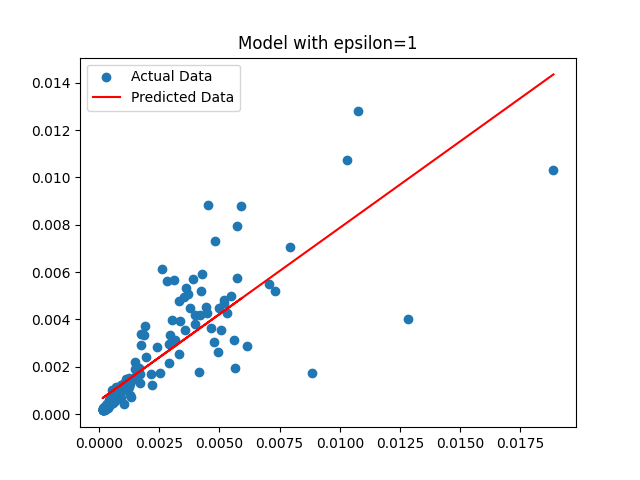
\includegraphics[width=.8\linewidth]{plots/epsilon_1}
            \caption{Caption for plot 1}
        \end{subfigure} \quad
        \begin{subfigure}[b]{0.3\textwidth}
            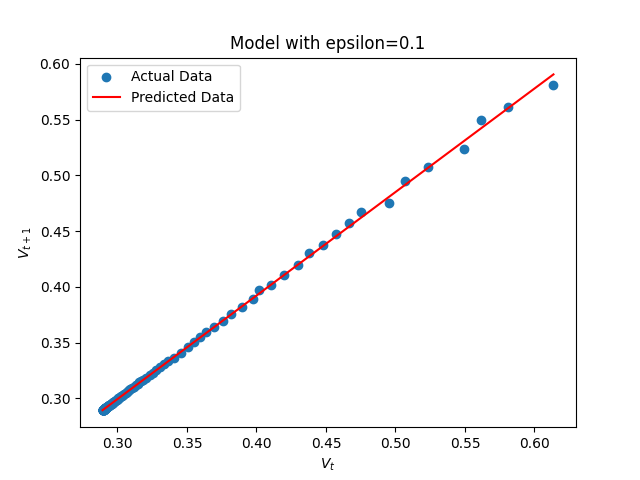
\includegraphics[width=.8\linewidth]{plots/epsilon_0.1}
            \caption{Caption for plot 2}
        \end{subfigure} \quad
        \begin{subfigure}[b]{0.3\textwidth}
            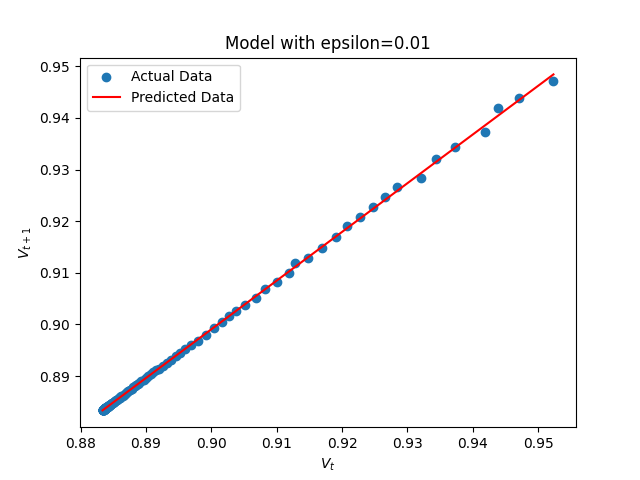
\includegraphics[width=.8\linewidth]{plots/epsilon_0.01}
            \caption{Caption for plot 3}
        \end{subfigure}\\
        \begin{subfigure}[b]{0.3\textwidth}
            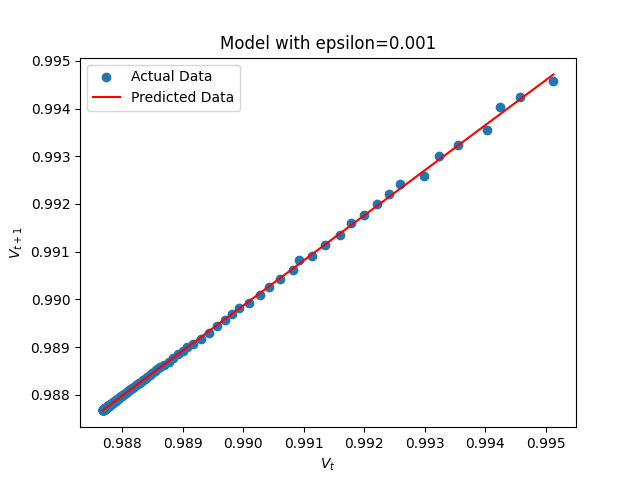
\includegraphics[width=.8\linewidth]{plots/epsilon_0.001}
            \caption{Caption for plot 4}
        \end{subfigure} \quad
        \begin{subfigure}[b]{0.3\textwidth}
            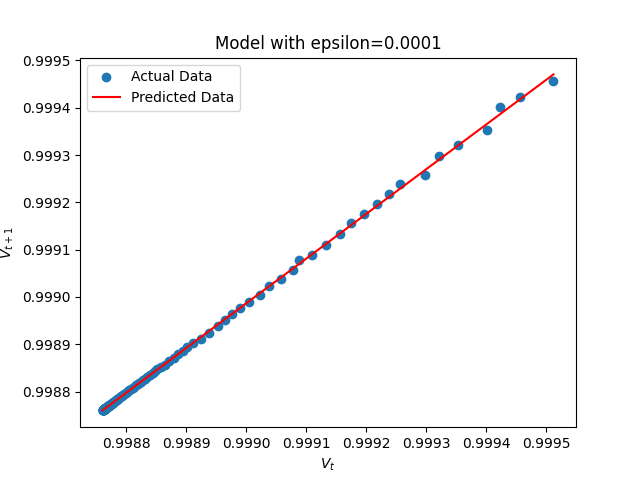
\includegraphics[width=.8\linewidth]{plots/epsilon_0.0001}
            \caption{Caption for plot 5}
        \end{subfigure}
        \caption{Overall caption for the figure}
    \end{figure}

    \subsection{GMM Regression}
    Let's consider the model:
    \begin{equation}
        N_{t} = \alpha_1 N_{t-1} + \alpha_2 N_{t-1}^{1 + \varepsilon} + U_t\label{eq:equation1}
    \end{equation}
    For a dataset of size $T$. We use GMM estimation, and since we have $3$ parameters, we need to use 3 moment conditions. We consider different UCMR:
    \begin{itemize}
        \item Assuming $U_t$ is orthogonal to $N_{t-1}$ and $N_{t-2}$ every period.
        \item Assuming $U_t$ is orthogonal to $N_{t-1}$ and $N^{\epsilon}_{t-1}$ every period.
    \end{itemize}

    \subsection{Case 1}
    Let's assume that $U_t$ is exogenous to $N_{t-1}$ and $N_{t-2}$ every period:
    \begin{equation}
        E[U_t|N_{t-2}, N_{t-1}] = 0
    \end{equation}
    Which implies the following unconditional moment restriction:
    \begin{equation}
        E \, \begin{bmatrix} 1  \\ N_{t-1} \\ N_{t-2} \end{bmatrix} U_t = 0
    \end{equation}
    In canonical form:
     \begin{equation}
        E \, g(N_{t-2}, N_{t-1}, N_t, \theta) = 0,
    \end{equation}
    Where:
    \begin{equation}
        g(N_{t-2}, N_{t-1}, N_t, \theta) =  \begin{bmatrix} 1 \\ N_{t-1} \\ N_{t-2}  \end{bmatrix} \left( N_{t} - \alpha_1 N_{t-1} - \alpha_2 N_{t-1}^{1 + \varepsilon} \right), \qquad \theta = \begin{bmatrix}
        \alpha_1 \\ \alpha_2 \\ \varepsilon \end{bmatrix}
    \end{equation}
    Bookkeeping:
    \begin{itemize}
        \item The estimator is just identified:
        \begin{equation}
            \dim \theta = \dim g = 3
        \end{equation}
        \item Function $g$ is non-linear in the parameters.
        \item Its Jacobian is:
        \begin{equation}
            D(\theta)= \frac{\partial g}{\partial \theta} =
            \begin{bmatrix}
                \frac{\partial g}{\partial \alpha_1} & \frac{\partial g}{\partial \alpha_2} & \frac{\partial g}{\partial \varepsilon}
            \end{bmatrix} = -
            \begin{bmatrix}
                N_{t-1} & N_{t-1}^{1+\varepsilon} & \alpha_2 N_{t-1}^{1+\varepsilon} \ln N_{t-1} \\
                N_{t-1}^{2} & N_{t-1}^{2+\varepsilon} & \alpha_2 N_{t-1}^{2+\varepsilon} \ln N_{t-1}\\
                N_{t-1} N_{t-2} & N_{t-1}^{1+\varepsilon} N_{t-2} & \alpha_2 N_{t-1}^{1+\varepsilon} N_{t-2} \ln N_{t-1}
            \end{bmatrix}
        \end{equation}
    \end{itemize}
    The estimator $\hat \theta$ is the minimizer:
    \begin{equation}
        \hat \theta = \arg \min_{\theta} \, E g^T(N_{t-2}, N_{t-1}, N_t, \theta)  \, S \, E g(N_{t-2}, N_{t-1}, N_t, \theta)
    \end{equation}
    for some weighting matrix $S$.

    \subsection{Numerical procedure}
    \subsubsection{Try 1}
    \begin{enumerate}
        \item Start by generating a random weighting matrix $S_0$.
        \item Make a $3\times 3$ grid of values for the parameters $(\alpha_1, \alpha_2, \varepsilon)$.
        \item Compute the sample equivalent of $m(\theta)=E g(N_t, N_{t+1}, \theta)$ for all points in the grid.
        \item Take $\hat \theta^{(1)}$ for which the target function $E g(N_t, N_{t+1}, \theta)  \, S \, E g^T(N_t, N_{t+1}, \theta)$ is minimum.
        \item Estimate the variance as the sample equivalent of $E g(N_t, N_{t+1}, \theta)  \, g^T(N_t, N_{t+1}, \theta)$ for $\theta = \hat \theta(1)$:
        \begin{equation}
            \hat V^{(1)}  = \frac{1}{T-1} \sum_{t=1}^{T-1} g(N_t, N_{t+1}, \hat \theta^{(1)}) g^T(N_t, N_{t+1}, \hat \theta^{(1)})
        \end{equation}
        \item Define a new weighting matrix $S^{(1)} = \left( \hat V^{(1)} \right)^{-1}$.
        \item Iterate until convergence, i.e., until $\left \vert \hat \theta^{(t+1)} - \hat \theta^{(t)} \right \vert_{i} < \Delta$ for each component $i=1,2,3$.
        \item Try with different starting matrices $S_0$ and different grids $(\alpha_1, \alpha_2, \varepsilon)$.
    \end{enumerate}
    \subsubsection{Try 2}
    \begin{enumerate}
        \item Start by generating a random weighting matrix $S_0$.
        \item Numerically solve the FOCs for $\theta$:
        \begin{equation}
            \hat D(\theta) \, S_0 \, \hat m (\theta) = 0
        \end{equation}
         the resulting $\hat \theta^{(1)}$ minimize the target function $E m\theta)  \, S \, m(\theta)$.
        \item Estimate the variance as the sample equivalent of $E g(N_t, N_{t+1}, \theta)  \, g^T(N_t, N_{t+1}, \theta)$ for $\theta = \hat \theta(1)$:
        \begin{equation}
            \hat V^{(1)}  = \frac{1}{T-1} \sum_{t=1}^{T-1} g(N_t, N_{t+1}, \hat \theta^{(1)}) g^T(N_t, N_{t+1}, \hat \theta^{(1)})
        \end{equation}
        \item Define a new weighting matrix $S^{(1)} = \left( \hat V^{(1)} \right)^{-1}$.
        \item Iterate until convergence, i.e., until $\left \vert \hat \theta^{(t+1)} - \hat \theta^{(t)} \right \vert_{i} < \Delta$ for each component $i=1,2,3$.
        \item Try with different starting matrices $S_0$ and different grids $(\alpha_1, \alpha_2, \varepsilon)$.
    \end{enumerate}






% \dot V(t) = -r\epsilon\, \left(V_0-K^{-1}\right)e^{-r\epsilon t}

For P-0 consider the stationary distribution as $t \to \infty $ and estimate t* as an average with that distribution